\section{Versuchsaufbau und Versuchdurchführung}

\begin{flushleft}
    Im den gesamten Versuch wird eine Drillachse, ein Metallstab, ein Winkelmesser, zwei Federwaagen ($0,2\,\unit{\newton}$ und $10\,\unit{\newton}$), 2 gleichschwere Gewichte,
    einen Styropor Zylinder, eine Holzkugel, eine Holzpuppe, eine kleine und eine große Schieblehre und eine Waage benötigt. Diese Objekte sind in Abbildung \ref{Abbildung1} zu sehen. \\
    
    \begin{figure}
        \centering
        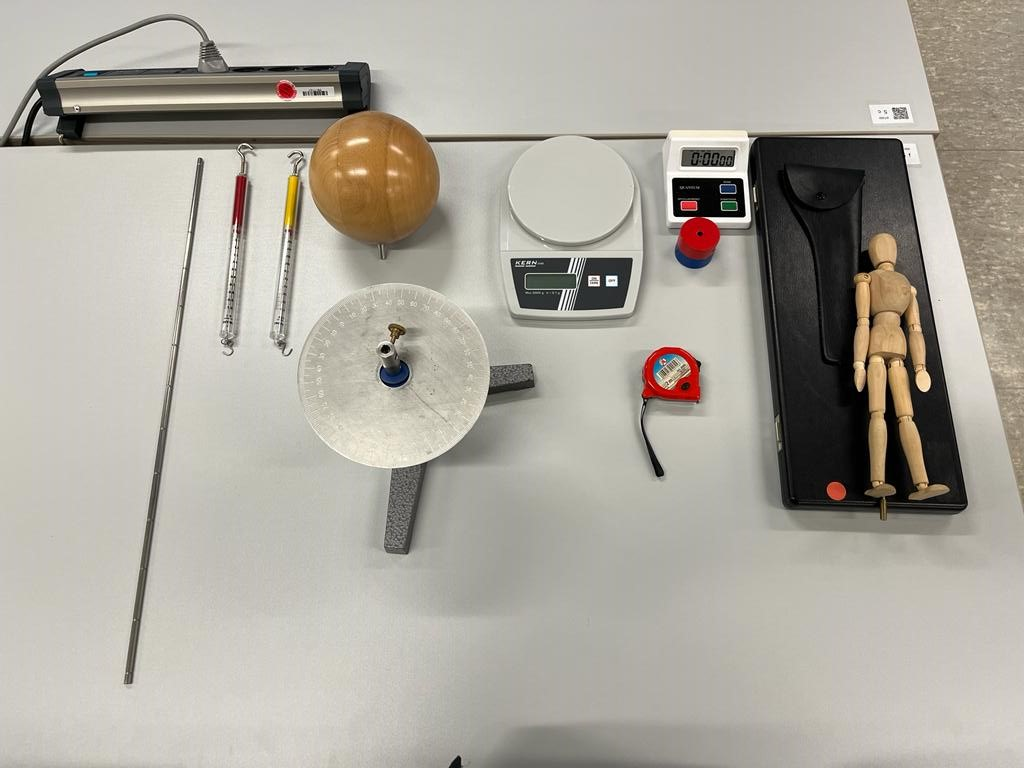
\includegraphics[height=80mm]{bilder/gesamt.jpeg}
        \caption{Die Abbildung aller Versuchsbauteilen. \label{Abbildung1}}
    \end{figure}
   

    Für den ersten Arbeitsauftrag wird an einer Drillachse die Mitte eines Metallstab befestigt. 
    Auf der Drillachse liegt ein Winkelmesser, welcher so eingestellt ist, dass die Ruhelage des Stabs bei $ 0 \unit{\degree}$ liegt. 
    An einer fest gewählten Stelle wird die Federwaage befestigt und waagerecht zum Stab gehalten. 
    Der Aufbau ist in Abbildung \ref{Abbildung2} zu sehen. 
    Danach wird der der Stab mithilfe der Federwaage um einen variablen Winkel $ \alpha $ ausgelenkt. 
    Die daraus resultierende Kraft, die auf der Federwaage angezeigt wird, gibt an wie viel Kraft benötigt wird um den Stab um den Winkel $ \alpha $ auszulenken.
    Der Winkel muss mindestens 10 mal geändert werden.
    Die daraus resultierenden Werte werden in Tabelle \ref{Tabelle1} festgehalten.\\

    \begin{figure}
        \centering
        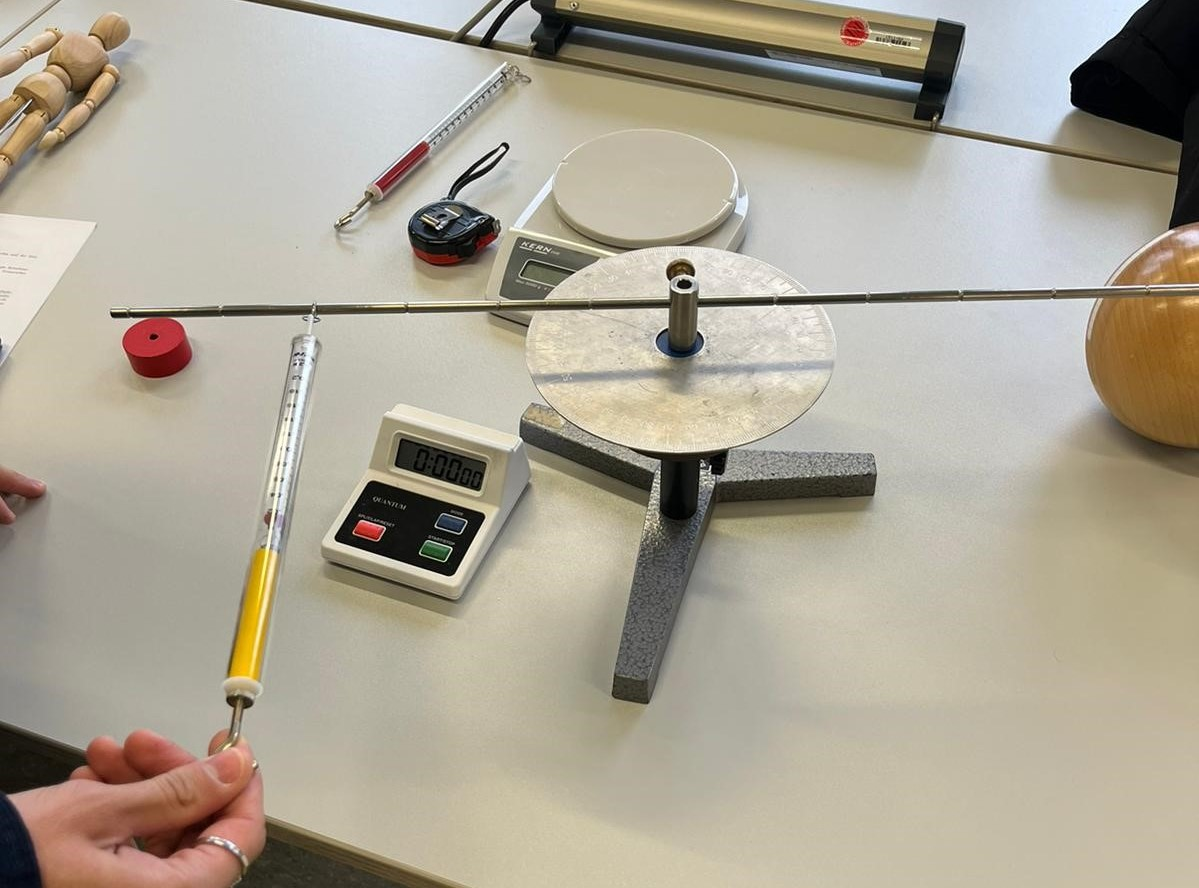
\includegraphics[height=70mm]{bilder/federwaage.jpeg}
        \caption{Der Aufbau für die Federwaage, welche am Stab befestigt ist. \label{Abbildung2}}
    \end{figure}

    \newpage

    Als nächstes wird die Federwaage mit zwei gleichschweren und gleichgroßen Gewichten ausgewechselt. 
    Jedes Gewicht wird auf einer Seite im selben Abstand befestigt. 
    Der Aufbau ist in Abbildung \ref{Abbildung3} zu sehen.
    Um das Eigenträgheitsmoment nun zu bestimmen wird diese Aufbaukonstruktion zum Schwingen gebracht. 
    Dies wird durch das auslenken um $180 \unit{\degree}$ des Stabes mit den Gewichten herbeigeführt. 
    Betrachtet wird eine ganze Schwingperiode. Eine ganze Schwingperiode ist vom Auslenken bis zum Maximumspunkt in Richtung Ursprungsauslenkung. 
    Hierbei werden die Abstände zur Drehachse verändert, wobei die Abstände der beiden Gewichte zur Drehachse auf beiden Seiten immer gleich sind. 
    Die daraus resultierenden Werte werden in Tabelle \ref{Tabelle2} festgehalten.  \\


    \begin{figure}
        \centering
        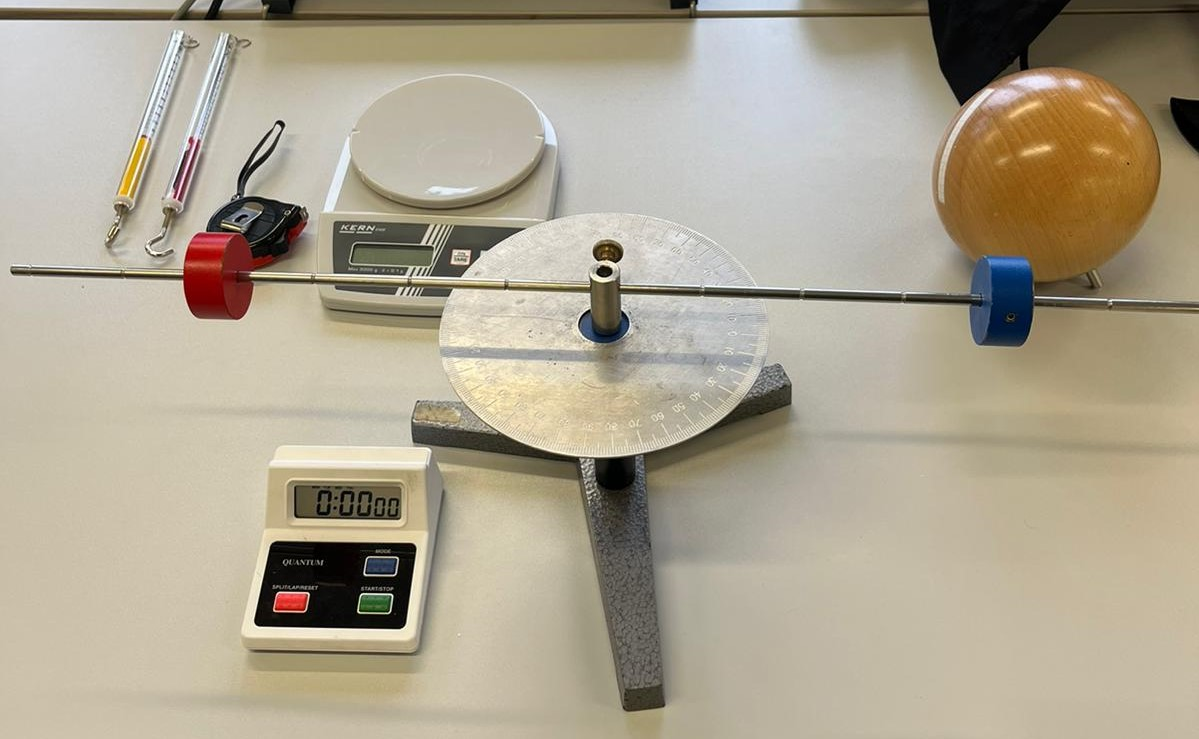
\includegraphics[height=60mm]{bilder/gewicht.jpeg}
        \caption{Der Aufbau der beiden Massen, welche am Stab befestigt sind. \label{Abbildung3}}
    \end{figure}

    \newpage
    
    Danach wird an einer Drillachse mit dem Winkelmesser einer von den beiden Körpern (Styroporzylinder, Holzkugel) befestigt. 
    Der Winkelmesser wird wieder so gelegt, dass die Markierung (welche auf den Objekten angezeichnet wurden) in Ruhelage bei $0 \unit{\degree}$ liegt. 
    Den Aufbau hierzu sieht man in Abbildung (\ref{Abbildung4a}) für den Styroporzylinder und in Abbildung (\ref{Abbildung4b}) für die Holzkugel.
    Die Durchführung für den Zylinder ist identisch zu der Kugel. 
    Man lenkt den Körper um $ 180 \unit{\degree} $ aus und misst wie lange der Körper für eine Schwingperiode benötigt.
    Man wiederholt dies jeweils fünf mal für jedes Objekt. \\
    Die daraus resultierenden Zeiten werden in Tabelle (\ref{Tabelle3}) für den Styroporzylinder und in Tabelle (\ref{Tabelle4}) für die Holzkugel festgehalten. \\

    \begin{figure}
        \begin{subfigure}{0.60\textwidth}
            \centering
            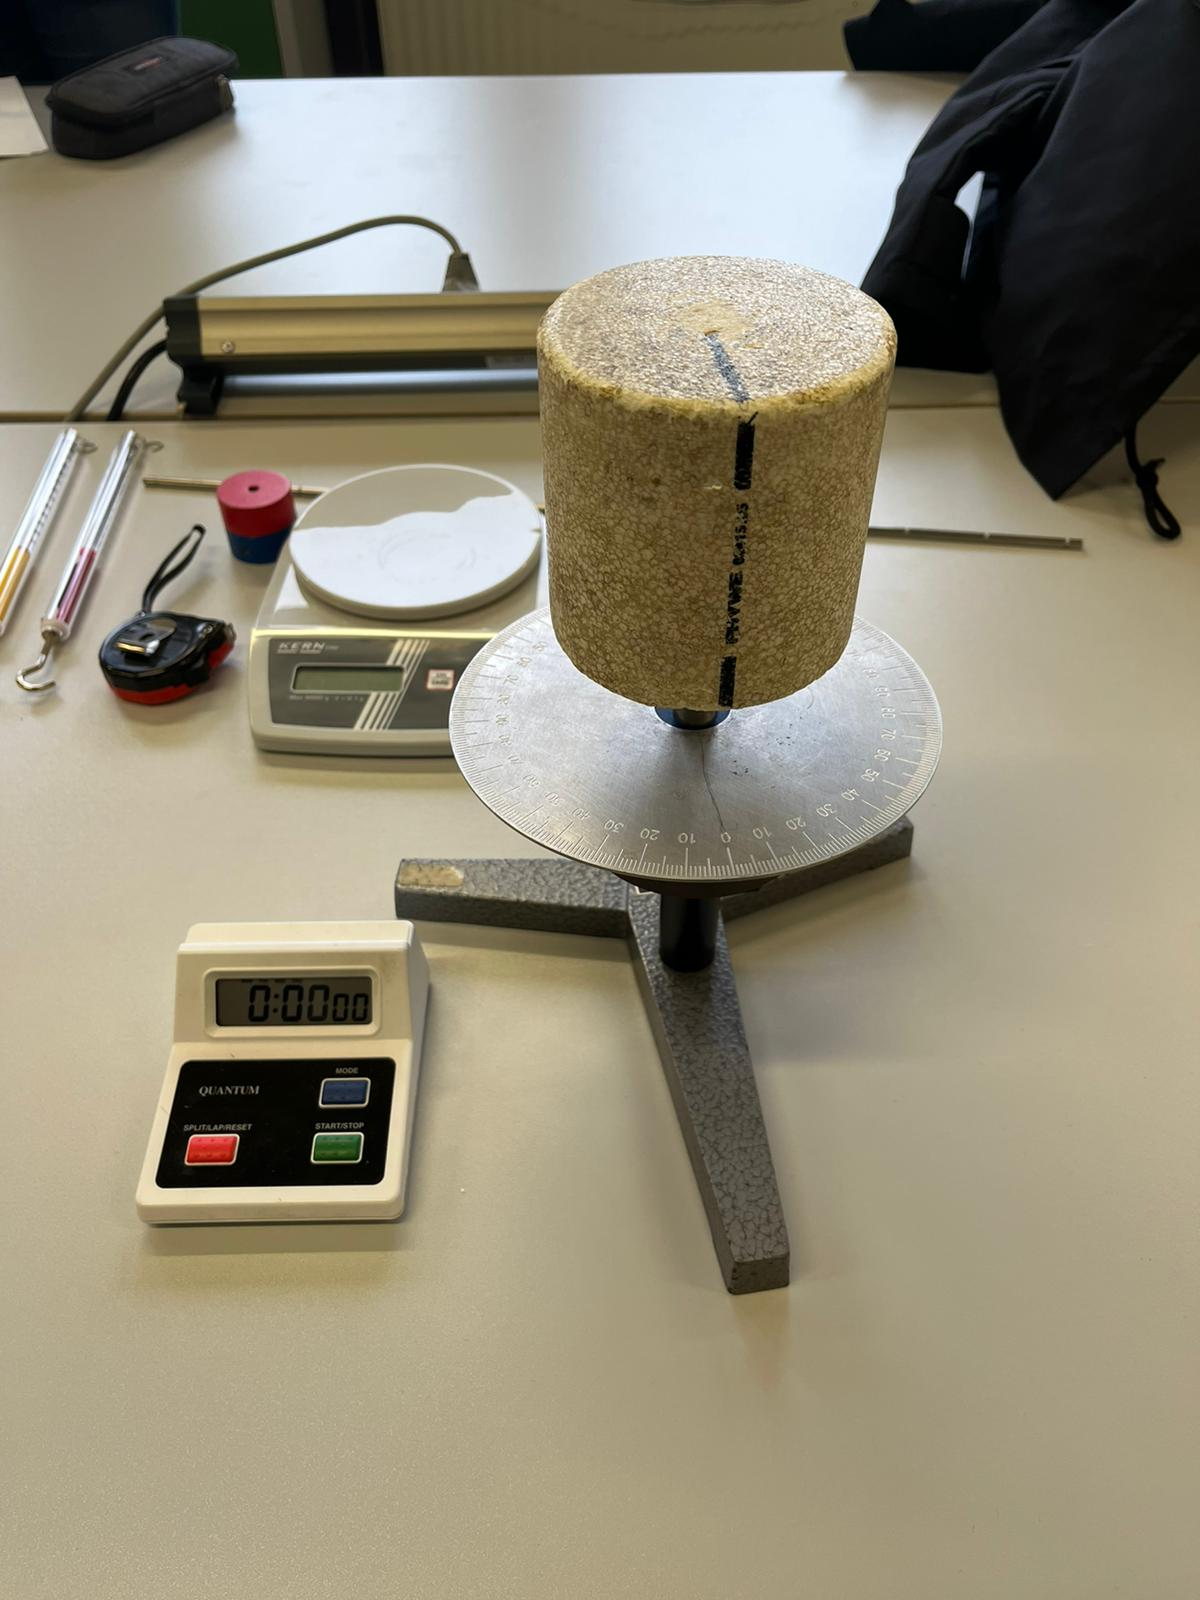
\includegraphics[width=53mm]{bilder/zylinder.jpeg}
            \caption{Der Aufbau zu dem Styroporzylinder an der Drillachse.} 
            \label{Abbildung4a}
        \end{subfigure}
        \hfill
        \begin{subfigure}{0.60\textwidth}
            \centering
            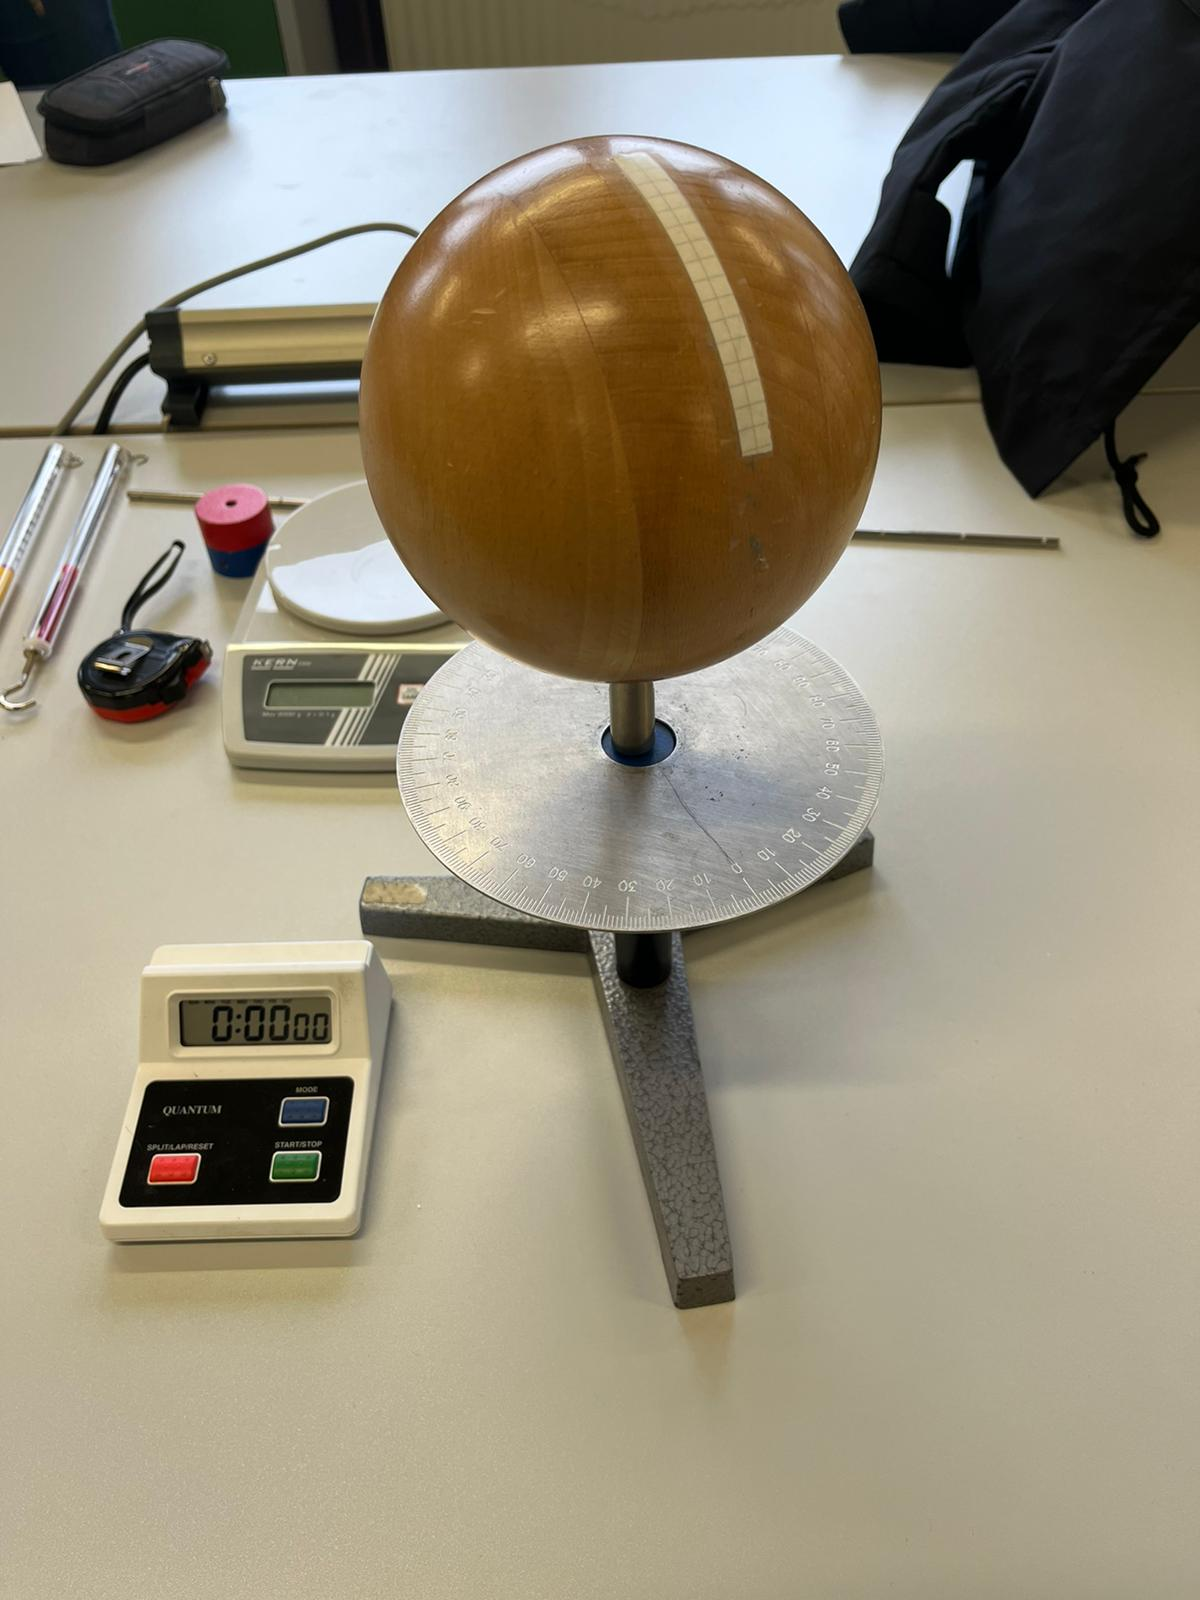
\includegraphics[height=73mm]{bilder/kugel.jpeg}
            \caption{Der Aufbau zu der Holzkugel an der Drillachse.} 
            \label{Abbildung4b}
        \end{subfigure}
        \caption{Die Darstellung der beiden Messkörper an der Drillachse. }
        \label{Abbildung4}
    \end{figure}

    Als letztes wird an der Drillachse eine Holzpuppe befestigt. 
    Diese hat zwei spezifische Haltungen. 
    Die erste ist mit den Armen am Körper und die zweite ist mit den Armen zur Seite hinausgestreckt.
    Den Winkelmesser legt man diesmal so an, dass die Mitte des Körpers in Ruhelage bei $0 \unit{\degree}$ liegt.
    Der Aufbau ist in Abbildung \ref{Abbildung5} zu sehen.
    Die Puppe wird dies nur um $ 90 \unit{\degree} $ ausgelenkt und die Schwingperiode gemessen.
    Dies wird für beide Haltungen jeweils 5 mal gemacht.
    Die daraus resultierenden Zeiten werden in Tabelle \ref{Tabelle6} für die Haltung eins und in Tabelle \ref{Tabelle7} für die Haltung zwei festgehalten.  \\

    \begin{figure}
        \begin{subfigure}{0.60\textwidth}
            \centering
            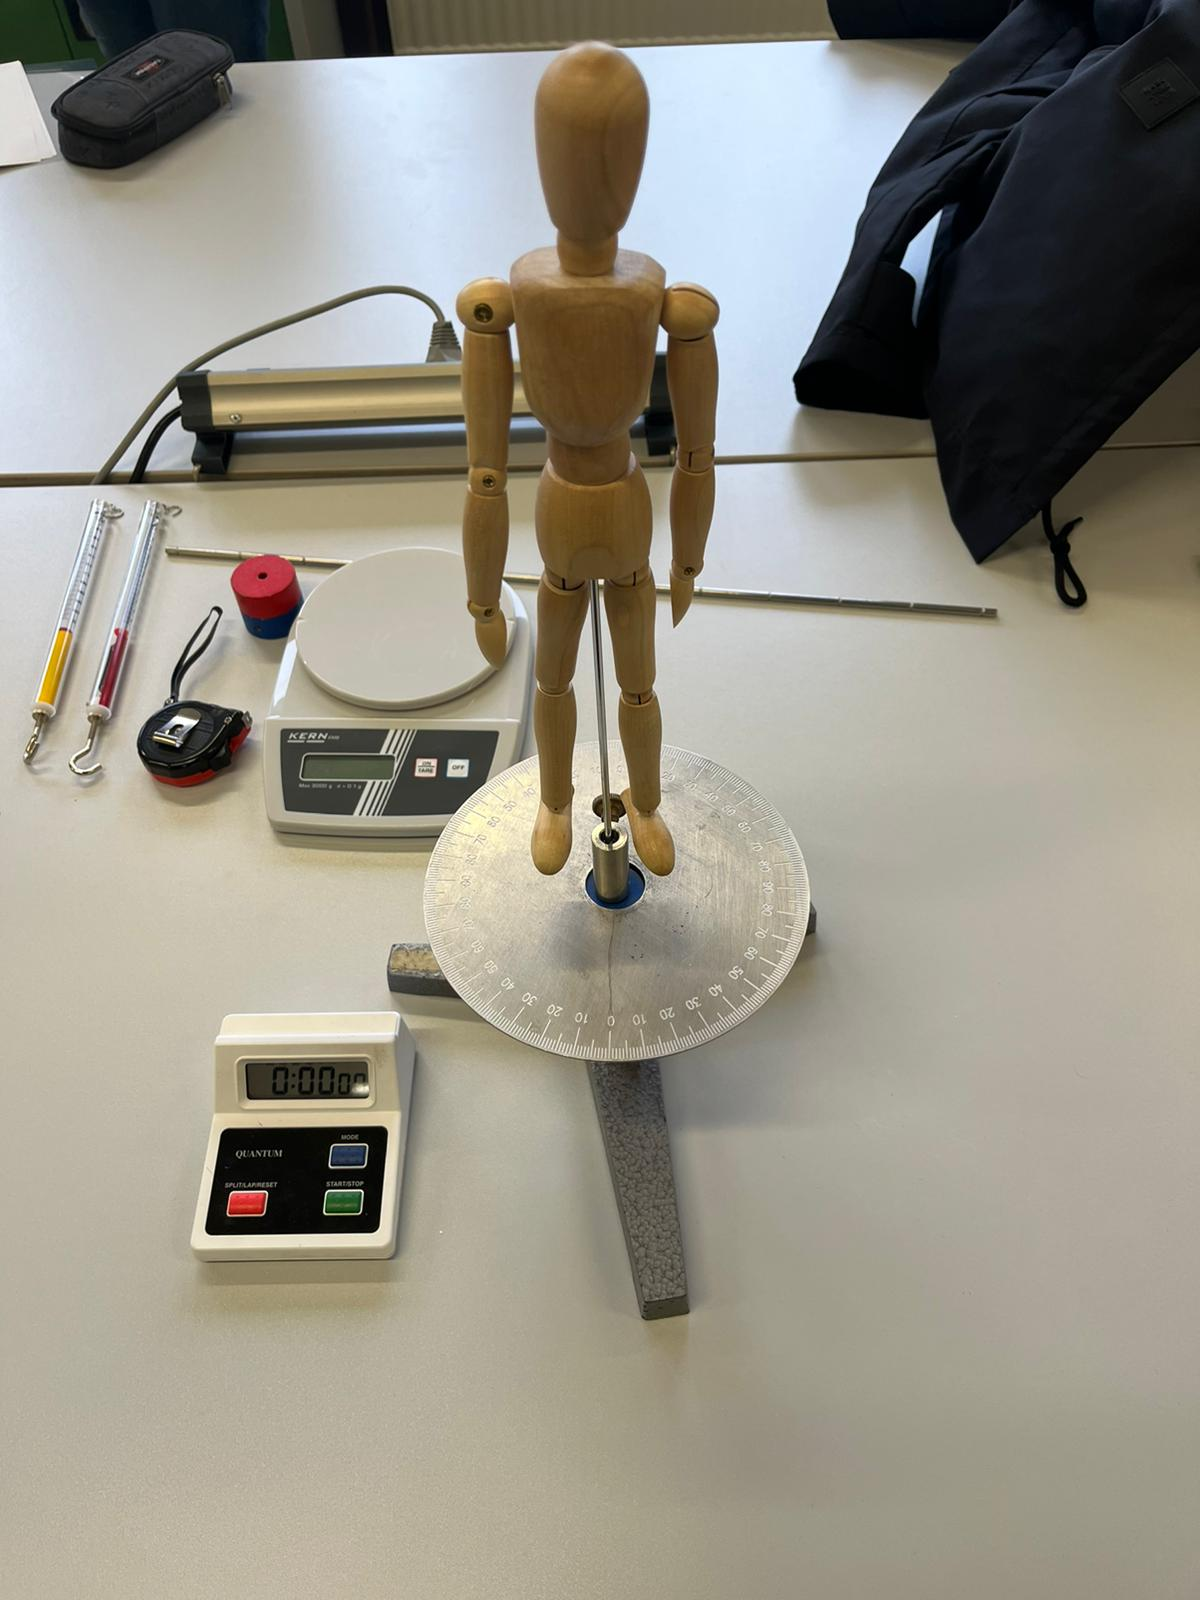
\includegraphics[width=53mm]{bilder/Haltung1.jpeg}
            \caption{Die Darstellung der ersten Haltung.} 
            \label{Abbildung5a}
        \end{subfigure}
        \hfill
        \begin{subfigure}{0.60\textwidth}
            \centering
            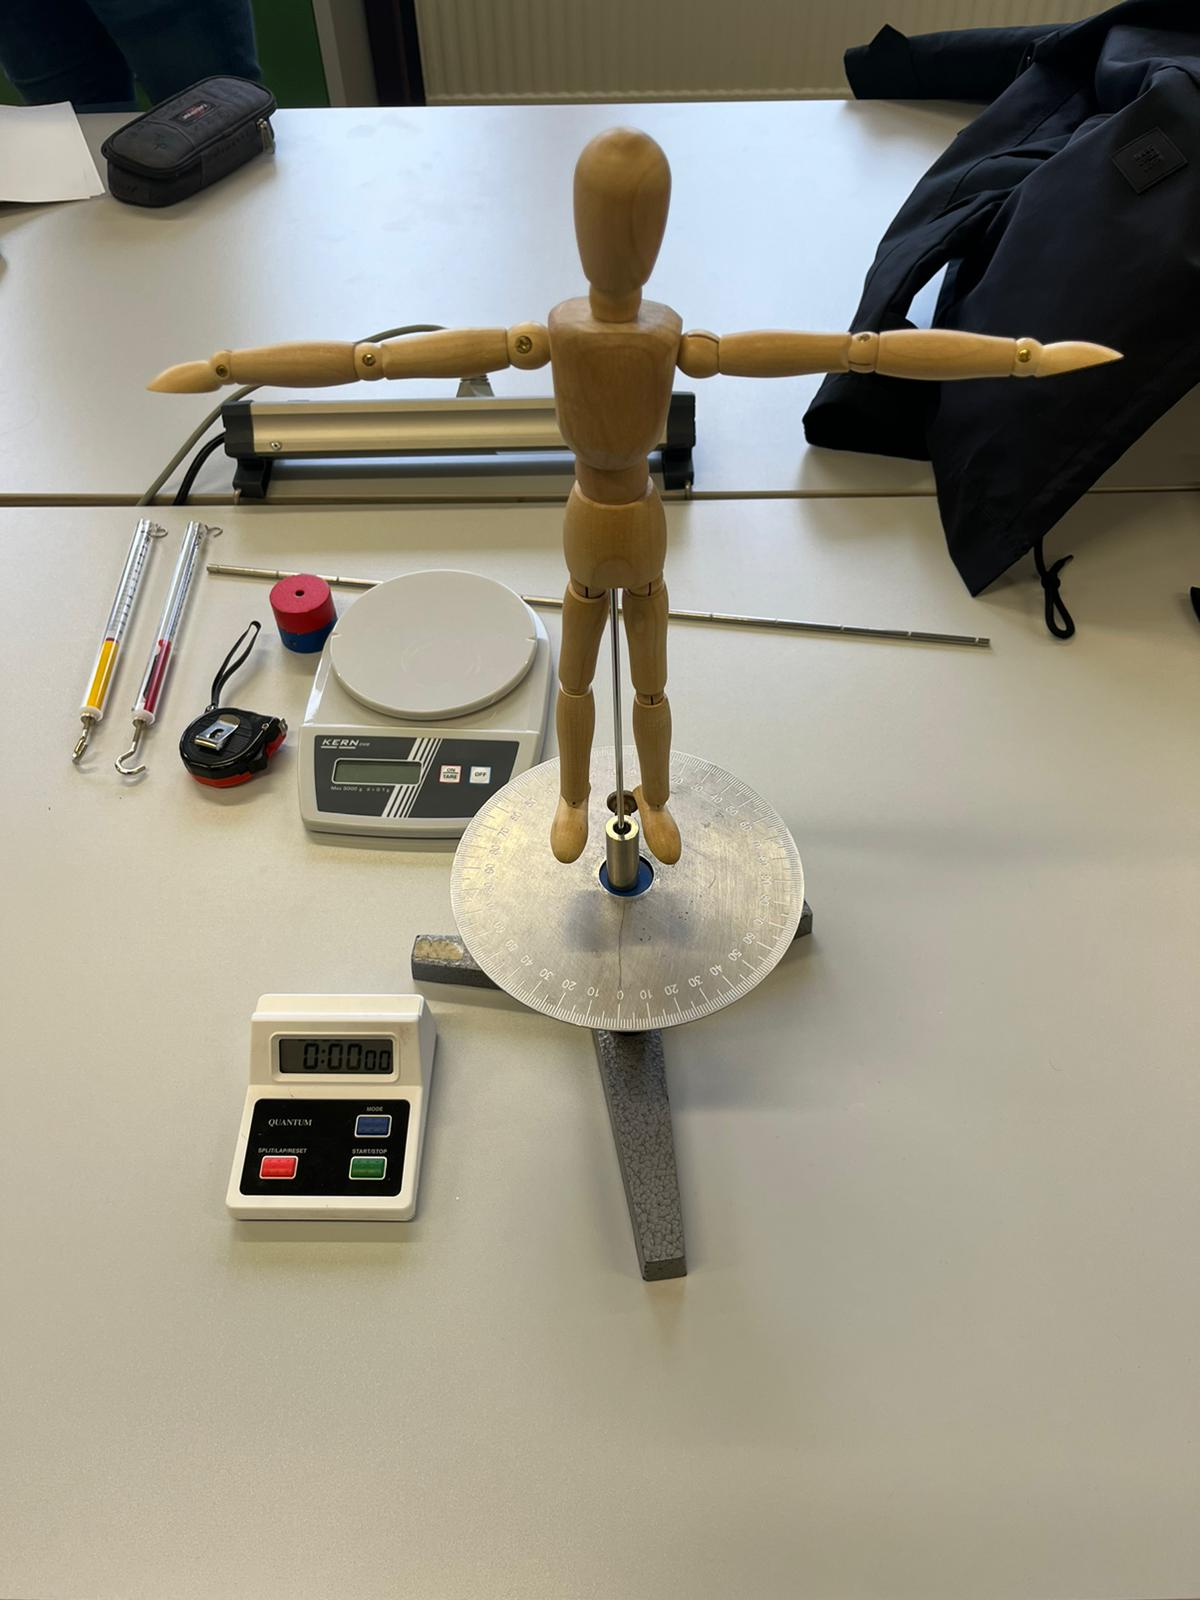
\includegraphics[height=71mm]{bilder/Haltung2.jpeg}
            \caption{Die Darstellung der zweiten Haltung.} 
            \label{Abbildung5b}
        \end{subfigure}
        \caption{Die Darstellung der beiden Haltungen der Holzpuppe. }
        \label{Abbildung5}
    \end{figure}

\end{flushleft}

